\documentclass[10pt]{article}
\usepackage[a4paper,margin=1in]{geometry}
\usepackage[T1]{fontenc}
\usepackage[utf8]{inputenc}
\usepackage{lmodern}
\usepackage{microtype}
\usepackage{amsmath,amssymb,amsthm}
\newtheorem{proposition}{Proposition}
\newcommand{\E}{\mathbb{E}}
\newcommand{\KL}{\mathrm{KL}}
\usepackage{booktabs}
\usepackage{graphicx}
\usepackage{xcolor}
\usepackage[numbers,sort&compress]{natbib}
\usepackage[colorlinks=true,allcolors=blue!50!black]{hyperref}
\newcommand{\thetastar}{\theta^{*}}

\title{What Is Another Sample Worth?\\
Exact Bayesian Grading for Agent Environments}

\author{Konsta Kiirikki \and Nikolas Juhava \and Qilun Li \and Atte Laakso\\[2pt]
Team 3-Sigma, Junction 2026}
\date{November 2026}

\begin{document}
\maketitle

\begin{abstract}
We build agent environments whose reward is computed from an exact Bayesian model rather than
from sampled outcomes. The exact grader gives zero for doing nothing, is strictly proper,
splits an agent's loss into bad experiments and bad inference, and supports a test for leaked
information. Using it, we find that frontier agents with code execution reach the reference on
all ten environments whose generative model is stated; our one early gap came from an
undisclosed model and closed (0.24 to 0.98) once we disclosed it. The gap reappears when the
model must be \emph{learned at a price}. On a credit desk whose score generator is hidden but
can be sampled at \$1 per draw, a simple reference scores 0.94--0.98 in expectation and every
agent we ran averages below it. The best agents decide within a few dollars of the true-model
optimum but buy two to five times more calibration data than it is worth.
\end{abstract}

\section{Introduction}

An agent that does science must choose experiments, update its beliefs, and decide when it
knows enough to act. Bayesian experimental design says how to do this optimally when the
data-generating model is known~\citep{lindley1956measure,chaloner1995bayesian,rainforth2024modern},
which makes such tasks attractive as agent environments: there is a reference that cannot be
beaten on average, so any shortfall is the agent's. We asked where a frontier agent with a
shell persistently scores below a fair reference for a reason that lies in the problem, not in
the task's wording. Our contributions are:
\begin{enumerate}
\item An exact grader for prediction and decision tasks, with guarantees (Section~\ref{sec:methods}).
\item Evidence that stated Bayesian problems are solved: across ten environments, agents with
code write exact inference and dynamic programs (Section~\ref{sec:stated}).
\item A task where the model is hidden but can be bought, on which every agent falls short,
and a decomposition showing the shortfall is in how much they learn, not how they decide
(Section~\ref{sec:blackbox}).
\end{enumerate}

\section{Related work}

BoxingGym~\citep{gandhi2025boxinggym} introduced simulators with an experiment-then-predict
protocol; two of our tasks are ports of its environments with a different grader.
DiscoveryWorld~\citep{jansen2024discoveryworld} and ChemGymRL~\citep{beeler2023chemgymrl} grade
open-ended discovery and procedure outcomes. Model Discovery Agent~\citep{murphy2026mda} and
BMD~\citep{yuh2026bmd} pair a language model with a numerical inference engine; our agents
build that engine themselves. Information-gain rewards have been used to train language models
with GRPO~\citep{shao2024deepseekmath,kriz2026amortizing,verma2026igft,li2026cigask}, usually with
a language-model likelihood; ours is the simulator, so the reward is exact. Pricing information
goes back to \citet{howard1966information}; \citet{frazier2010paradoxes} show that its value is
not concave in the number of measurements, which is why one-step reasoning fails. Acting while
learning is dual control~\citep{feldbaum1960dual,duff2002optimal}. Our prediction reward is a
proper scoring rule~\citep{gneiting2007strictly} in expectation, the leak test is a posterior
predictive check~\citep{gelman1996posterior}, and the decision reward uses the advantage
decomposition of \citet{kakade2002approximately}.

\section{Methods}
\label{sec:methods}

\paragraph{Environments.} Each environment has hidden state drawn from a public prior, a menu of
costly observations, and a grader with an exact model of what they imply
(Table~\ref{tab:envs}).

\begin{table}[t]
\centering\small
\begin{tabular}{p{3.4cm}p{6.2cm}p{4.2cm}}
\toprule
Problem & Environment & Exact computation \\
\midrule
Parameter estimation & Hyperbolic discounting, location finding, dose response & Particle posterior \\
Fault diagnosis & Chemistry lab (7 faults) & Enumeration \\
Mechanism discrimination & Wet lab; likelihood-free gene lab & Finite state projection \\
Population learning & Hierarchical lab & Conjugate updates \\
Causal discovery & Random-DAG lab (29{,}281 graphs); optogenetics lab & Enumeration \\
Planning, decisions & Diagnostic planning; blackjack with hidden shoe & Dynamic program \\
Optimal stopping & Credit desk, model stated & Dynamic program \\
\textbf{Priced model learning} & \textbf{Credit desk, model hidden} & DP under true generator \\
\bottomrule
\end{tabular}
\caption{Environments. The last row is the submission task.}
\label{tab:envs}
\end{table}

\paragraph{Prediction reward.} The agent runs up to 10 experiments, then submits a predictive
distribution $q$ for 30 evaluation designs. With $S(q;\theta)$ the expected log score under
true parameters $\theta$ (computed, not sampled),
\begin{equation}
R(q) = \mathrm{clip}_{[0,1]}\!\left(
\frac{S(q;\thetastar) - S(p_{0};\thetastar)}{S(p_{\thetastar};\thetastar) - S(p_{0};\thetastar)}\right),
\label{eq:reward}
\end{equation}
so the prior predictive $p_0$ scores 0 and knowing $\thetastar$ scores 1. The gap to a
reference that designs greedily by expected information gain splits exactly into \emph{design
loss} $S_\mathrm{ref} - S(p_D)$ and \emph{inference loss} $S(p_D) - S(q)$, where $p_D$ is the
posterior predictive given the agent's data $D$. The \emph{leak test} compares
$T(\theta) = S(q;\theta) - S(p_D;\theta)$ at $\thetastar$ with its value at 400 posterior draws;
p-values are combined over a batch with Fisher's method and a two-sided Kolmogorov--Smirnov
statistic.

\paragraph{Decision reward.} The grader solves the dynamic program (DP) for the true model and
credits a trajectory with
\begin{equation}
\hat V = V^{*}(s_0) - \textstyle\sum_{t} \big[ V^{*}(s_t) - Q^{*}(s_t, a_t) \big],
\label{eq:vhat}
\end{equation}
the optimal value minus the advantage given up at each step.

\paragraph{Guarantees.} For agents whose submission depends on $\theta$ only through their own
data (``no leak''), we prove in Appendix~\ref{app:proofs}: the score is strictly proper; no
submission beats $p_D$ in expectation, and inference loss is exactly $\E[\KL(p_D\|q)]$; the
expected reward of $p_D$ is the mutual information between data and outcome; exact grading has
lower variance than grading against a sampled outcome; the leak test is valid at every level;
and $\hat V$ is an unbiased estimate of the policy's expected profit, at most $V^{*}(s_0)$, and
exactly $V^{*}(s_0)$ for an optimal policy whatever the luck. The guarantees hold for the score;
the clipped and normalised rewards inherit them only up to clipping.

\paragraph{The black-box credit desk.} The agent underwrites 20 applicants. Each belongs to one
of six risk segments with stated default probabilities and prior; approving pays the expected
payoff for the true segment (margin \$1{,}000, loss given default \$16{,}000). Before deciding,
the agent may buy up to eight live checks of three kinds at \$20 each, each returning a band of a
score. The task states that score $=$ location(segment) $+$ symmetric noise specific to the
check, but hides the locations and the noise families (Gaussian, Student-$t_3$ or Cauchy, at
least one Cauchy per desk). A sandbox returns raw scores for synthetic applicants of a known
segment at \$1 per draw, up to 1{,}000. With $V = \sum_i \hat V_i - \text{sandbox spend}$,
\begin{equation}
\text{reward} = \mathrm{clip}_{[0,1]}\big((V - V_0)/(\bar V_{\mathrm{ref}} - V_0)\big),
\end{equation}
where $V_0$ is the value of deciding from the prior and $\bar V_\mathrm{ref}$ the reference's
expected total over 200 sandbox datasets. The \emph{reference} uses only the agent's tools: 12
draws per (segment, check) cell (\$216), per-cell medians, pooled symmetrised residuals,
bootstrap-averaged band tables, and the exact DP. We kept six of 20 screened desks on which the
reference has mean 0.94--0.98 and SD $\le 0.12$, and shortcuts score at most 0.8 in
expectation: no calibration 0.00--0.37, Gaussian fit 0.53--0.73, one-step lookahead
0.07--0.30, buying all 1{,}000 draws 0.39--0.52. Doing nothing scores 0.

\paragraph{Agents.} Agents run in Harbor with a Python shell; the environment is an MCP server
in a separate container, and a verifier calls a token-protected grading endpoint. We ran Claude
Code (Opus~5.5, Sonnet~5.5), Codex (GPT-6 Luna, GPT-5.6 Terra) and OpenCode (GPT-5.6 Terra,
Gemini~4 Argon, Kimi K3.1 Pro, MiniMax-M3, DeepSeek V4.1 Flash, Nemotron~3 Ultra, Gemma~4 26B).
Comparisons across agents confound model and harness.

\section{Results}

\subsection{The exact grader}
\label{sec:results1}

Under a naive grader that scores point predictions against one sampled outcome, doing nothing
earns 0.919 on hyperbolic discounting and an overconfident policy ties the reference
(Table~\ref{tab:e1}). Under Eq.~\eqref{eq:reward} both fail, and showing that the reference
beats random design takes 4--5 paired seeds instead of 14--18. Seven attacks using only
legitimate information (point estimates, sharpening, blunting, one design) never beat the
reference. Blending 10\% of the truth into predictions is flagged in every batch of 30
episodes; the best evasion we found gains $+0.04$ to $+0.05$.

\begin{table}[t]
\centering\small
\begin{tabular}{lcccc}
\toprule
 & \multicolumn{2}{c}{Hyperbolic} & \multicolumn{2}{c}{Location} \\
\cmidrule(lr){2-3}\cmidrule(lr){4-5}
Policy & Naive & Bayes & Naive & Bayes \\
\midrule
Bayesian reference    & 0.981 & 0.949 & 0.695 & 0.990 \\
Random design         & 0.954 & 0.539 & 0.549 & 0.753 \\
Stop early (1 exp.)   & 0.947 & 0.467 & 0.125 & 0.216 \\
Do nothing            & 0.919 & 0.000 & 0.000 & 0.000 \\
Overconfident         & 0.981 & 0.520 & 0.695 & 0.000 \\
\bottomrule
\end{tabular}
\caption{Scripted policies, 400 seeds each, under a naive and the exact grader.}
\label{tab:e1}
\end{table}

\subsection{Stated models are solved}
\label{sec:stated}

Our first agent gap was an artefact. As ported, the hyperbolic-discounting task did not state
the choice model or priors, which the reference knew. Disclosing them took Claude Code with Opus
from 0.24 to 0.98 and Codex with GPT-6 Luna from 0.06 to 0.87. We then tried to rebuild the gap
honestly with harder stated problems, each calibrated so that a named shortcut loses clearly
(Table~\ref{tab:stated}). In every environment the agent wrote exact inference, and where
needed an exact DP, and reached the reference.

\begin{table}[t]
\centering\small
\begin{tabular}{p{3.6cm}p{4.6cm}p{5.6cm}}
\toprule
Environment & Shortcut it was built against & Claude Code with Opus 5.5 \\
\midrule
Chemistry lab & Uninformative experiments & Gap $+0.006$ nats, 15 trials \\
Hierarchical lab & No / complete pooling & Exact inference, 4 trials \\
Random-DAG, optogenetics & Correlation as causation & Inference gap 0 in 7 of 8 trials \\
Diagnostic planning & Greedy tests (1.06 vs.\ DP 1.71) & 1.69 over 8 trials \\
Likelihood-free gene lab & Moment matching, ABC & 0.93, 1.00 (reference 0.88) \\
Blackjack, hidden shoe & Card-counting heuristics & Zero regret, 4 of 4 trials \\
Credit desk, model stated & One-step lookahead (0.19) & 1.0 in 3 of 3 trials \\
\bottomrule
\end{tabular}
\caption{Stated-model environments. With the two disclosed prediction tasks, these make ten.}
\label{tab:stated}
\end{table}

Without code execution the same models are less reliable. Gemini~4 Argon's stated posteriors
are close to exact (mean KL 0.010 under Cauchy noise), but it stops too early when stakes are
high: on a diagnosis task its share of the achievable value falls from 0.92 at penalty/reward
ratio 0.25 to 0.13 at 16, and 93 of 102 early stops match one-step lookahead. These errors
vanish once the agent can write the DP. They motivated the next task.

\subsection{The black-box credit desk}
\label{sec:blackbox}

\begin{table}[t]
\centering\footnotesize\setlength{\tabcolsep}{4pt}
\begin{tabular}{llccccccc}
\toprule
 & & & Timed & \multicolumn{2}{c}{Reward} & Sandbox & Play & Checks per \\
\cmidrule(lr){5-6}
Agent & Harness & $n$ & out & Mean & Range & spend (\$) & loss (\$) & applicant \\
\midrule
Reference (oracle run) & oracle & 6 & 0 & 0.97 & 0.82--1.00 & 216 & 100 & 2.22 \\
\midrule
Claude Opus 5.5 & Claude Code & 3 & 0 & 0.79 & 0.71--0.86 & 540 & 25 & 1.75 \\
Claude Sonnet 5.5 & Claude Code & 6 & 0 & 0.71 & 0.47--0.98 & 318 & 396 & 1.48 \\
Gemini 4 Argon & OpenCode & 4 & 3 & 0.28 & 0.00--1.00 & 159 & 122 & 1.85 \\
Kimi K3.1 Pro & OpenCode & 3 & 1 & 0.43 & 0.15--0.61 & 950 & 10 & 1.98 \\
MiniMax-M3 & OpenCode & 3 & 2 & 0.20 & 0.00--0.59 & 790 & 51 & 2.25 \\
DeepSeek V4.1 Flash & OpenCode & 6 & 0 & 0.27 & 0.00--0.45 & 1000 & 102 & 2.30 \\
GPT-5.6 Terra & OpenCode & 6 & 0 & 0.10 & 0.00--0.35 & 900 & 973 & 1.40 \\
Nemotron 3 Ultra & OpenCode & 4 & 0 & 0.01 & 0.00--0.05 & 900 & 1326 & 0.68 \\
\bottomrule
% generated by v2_table.py; ends with the bottom rule
\end{tabular}
\caption{Black-box credit desk, one Harbor trial per desk per agent. Timed-out trials (45-minute
limit) count undecided applicants as declined. The last three columns are medians over finished
trials. \emph{Play loss}: true-model DP value minus the agent's value before sandbox costs.}
\label{tab:v2}
\end{table}

\begin{figure}[t]
\centering
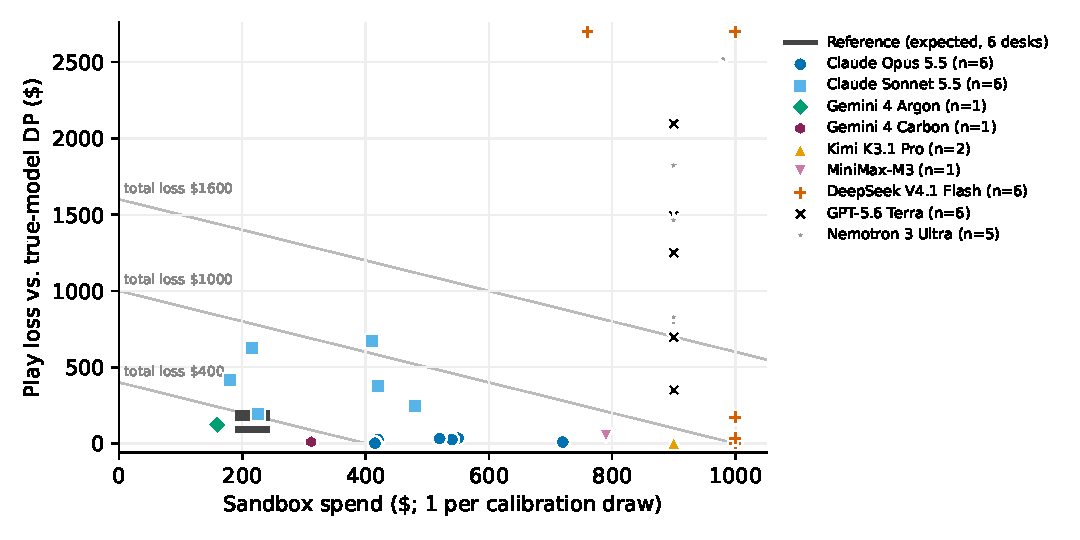
\includegraphics[width=0.9\linewidth]{fig_v2}
\caption{Finished trials: what each agent paid to learn the generator (horizontal) against what
its decisions then lost to the true-model DP (vertical). Grey lines join equal total loss.
Bars mark the reference's expectation per desk.}
\label{fig:v2}
\end{figure}

Every agent averages below the reference (Table~\ref{tab:v2}, Figure~\ref{fig:v2}), and the
grader shows where the money went. \emph{Opus~5.5 plays near-optimally but overbuys}: it lost only
\$9--\$32 to the true-model DP, where the reference loses \$86--\$200, but bought 520--720 draws
against 216, an extra \$300--\$500 that buys back at most about \$170. It identified the noise
families correctly and ran an exact DP, but fixed its budget by convention (20 draws per cell)
rather than pricing a further draw. Kimi and DeepSeek bought close to the 1{,}000 cap.
\emph{Sonnet~5.5 spends moderately but decides worse}, running fewer live checks than the
reference. \emph{GPT-5.6 Terra and Nemotron spend heavily and decide poorly}, several trials
ending below the value of declining everyone. \emph{Argon and MiniMax mostly ran out of time};
the instruction did not state the limit, so these scores say little about their decisions. One
Argon trial scored 1.0 after simulating how regret falls with draws per cell before buying 159;
it was the only agent that priced its calibration.

\subsection{Training small models}

On rows asking for the most informative experiment, labelled by exact expected information
gain, supervised fine-tuning and GRPO lift every Gemma~4 size (E2B to 26B) above its base and a
shuffled-reward control on unseen task families; for E4B, from 0.29 to 0.57 (GRPO) and 0.59
(supervised). On hyperbolic discounting E4B goes from 0.000 to 0.362 with supervised
fine-tuning and to 0.499 with GRPO. None of this is yet on the submission task.

\section{Discussion}

The agents' statistics and planning are strong; what they lack is treating ``how much should I
learn?'' as a decision with a computable answer. The reference's 12 draws per cell was found by
simulation with tools every agent has. This is the myopia about the value of information that
the text-only experiments showed for a single check, moved to a level where writing a DP for the
stated problem does not remove it, because the stated problem does not include it.

\paragraph{Limitations.} The black-box results are at most six trials per agent on one task
family, with different harnesses; for two agents most trials hit the time limit, which the
instruction did not state. Two trials came within 0.03 of the reference, so the gap is one of
frequency. A prompt telling agents to price calibration would probably narrow it. The reference
is good, not optimal. The verifier shares a container with the agent, and the sandbox stream is
fixed per desk, so baselines are compared in expectation. Stated-model results rest on 2--15
trials per environment.

\section{Conclusion}

When the grader knows the simulator, the exact posterior and value function turn a noisy
benchmark into an environment with a provable ceiling, a zero for doing nothing, and a
per-step account of where an agent lost. That account showed that our first gap was created by
withheld information, that frontier agents with code solve stated Bayesian problems, and that
agents which infer and plan almost perfectly still misjudge how much learning is worth.

\section*{Use of AI}

This work was produced at a 48-hour hackathon with heavy use of AI coding agents. Claude Code
(Anthropic; Claude Fable 5.2 and Claude Opus 5.5) wrote most of the code, ran and analysed the
experiments, searched the literature and drafted this manuscript under the direction of the
human authors, who chose the question and experiments, reviewed the results, and take
responsibility for the content. The models named in the results were experimental subjects.

\bibliographystyle{unsrtnat}
\bibliography{refs}

\appendix
\section{Proofs}
\label{app:proofs}

Let $\theta \sim \pi$, let the agent choose designs from its history and private randomness $U$
independent of $\theta$, and let $q$ have \emph{no leak}: conditionally independent of $\theta$
given $D$ and the evaluation design $x$. Write $p_\theta = p(\cdot\mid x,\theta)$ and
$p_D = \int p_\theta\, p(\theta\mid D)\,d\theta$.

\begin{proposition}[Proper]\label{prop:proper}
$S(p_\theta;\theta) - S(q;\theta) = \KL(p_\theta\|q) \ge 0$, with equality only if $q = p_\theta$.
\end{proposition}
\emph{Proof.} The difference is $\E_{Y\sim p_\theta}[\log p_\theta(Y) - \log q(Y)]$; apply Gibbs'
inequality. \qed

\begin{proposition}[Nobody beats the posterior]\label{prop:bayes}
$\E[S(p_D;\theta)] - \E[S(q;\theta)] = \E[\KL(p_D\|q)] \ge 0$.
\end{proposition}
\emph{Proof.} Each design is a function of the past data and $U$, so the joint density of
$(\theta, D)$ given $U$ is $\pi(\theta)\prod_t p(y_t\mid x_t,\theta)$ times factors free of
$\theta$; hence $\theta\mid(D,U,x)\sim p(\theta\mid D)$. Conditioning fixes $q$, and
$\E[S(q;\theta)\mid D,U,x] = \int p_D(y)\log q(y)\,dy$. Subtract the same identity with
$q=p_D$ and take expectations. \qed

\begin{proposition}[Information]\label{prop:info}
$\E[S(p_D;\theta) - S(p_0;\theta)] = I(Y;D)$.
\end{proposition}
\emph{Proof.} By the identity above the conditional expectation is $\KL(p_D\|p_0)$, whose mean
over $D$ is $I(Y;D)$ since $Y\mid D\sim p_D$ and $Y\sim p_0$. \qed

\begin{proposition}[Variance]\label{prop:var}
If $\hat S = \log q(Y)$ with $Y\sim p_{\thetastar}$, then $\E\hat S = \E S$ and
$\mathrm{Var}(S)\le\mathrm{Var}(\hat S)$.
\end{proposition}
\emph{Proof.} $S = \E[\hat S\mid\thetastar,q]$; apply the law of total variance. \qed

\begin{proposition}[Leak test]\label{prop:ppc}
For $\tilde\theta_1,\dots,\tilde\theta_m$ i.i.d.\ from $p(\theta\mid D)$ and any statistic $T$
of $(D,q,x)$, the p-value $(1+\#\{i: T(\tilde\theta_i)\ge T(\thetastar)\})/(m+1)$ satisfies
$\Pr(p\le\alpha)\le\alpha$ under no leak.
\end{proposition}
\emph{Proof.} Given $(D,q,x)$, $\thetastar$ and the $\tilde\theta_i$ are i.i.d., so the $m+1$
values of $T$ are exchangeable and $T(\thetastar)$ is among the $\lfloor\alpha(m+1)\rfloor$
largest with probability at most $\alpha$. \qed

\begin{proposition}[Advantage grading]\label{prop:adv}
In a finite-horizon problem with hidden state $h$, belief states $s_t$ and optimal values
$V^{*}, Q^{*}$ of the belief process, for any policy using only its history and independent
randomness: (i) $\E[\hat V]$ is the policy's expected total reward; (ii) $\hat V\le V^{*}(s_0)$,
with equality iff every action was optimal.
\end{proposition}
\emph{Proof.} As above, $h\mid(H_t,U)\sim s_t$, so with $\bar r(s,a)=\E_{h\sim s}r(h,a)$ we have
$Q^{*}(s_t,a_t)=\bar r(s_t,a_t)+\E[V^{*}(s_{t+1})\mid s_t,a_t]$. Substituting into
Eq.~\eqref{eq:vhat} gives $\hat V=\sum_t\bar r(s_t,a_t)-\sum_t(V^{*}(s_{t+1})-\E[V^{*}(s_{t+1})\mid
s_t,a_t])$; the second sum is a martingale difference with mean zero, which gives (i). Each
bracket in Eq.~\eqref{eq:vhat} is non-negative since $V^{*}=\max_a Q^{*}$, which gives (ii). \qed

\end{document}
